\chapter{Fundamentos teóricos para el desarrollo del proyecto}\label{cap:Fundamentos}

En este capítulo, enmarcado dentro de la primera fase de investigación y recopilación de información, enumeraremos aquellos aspectos cruciales para entender el resto del trabajo, que se han estudiado y analizado durante el desarrollo de este trabajo.

\section{Descripción técnica de Wazuh}

Wazuh es una \textbf{plataforma opensource de ciberseguridad}. Esto significa que \textbf{contiene distintos módulos que engloban muchas de las funcionalidades típicas de herramientas de seguridad defensivas}. 

Por ejemplo, Wazuh puede ser utilizado como un \textbf{\gls{siem}}, como un \textbf{\gls{HIDS}}, como una herramienta de monitorización de \textbf{integridad de ficheros}, entre otras funciones.

\begin{figure}[!hbt]
  \centering
  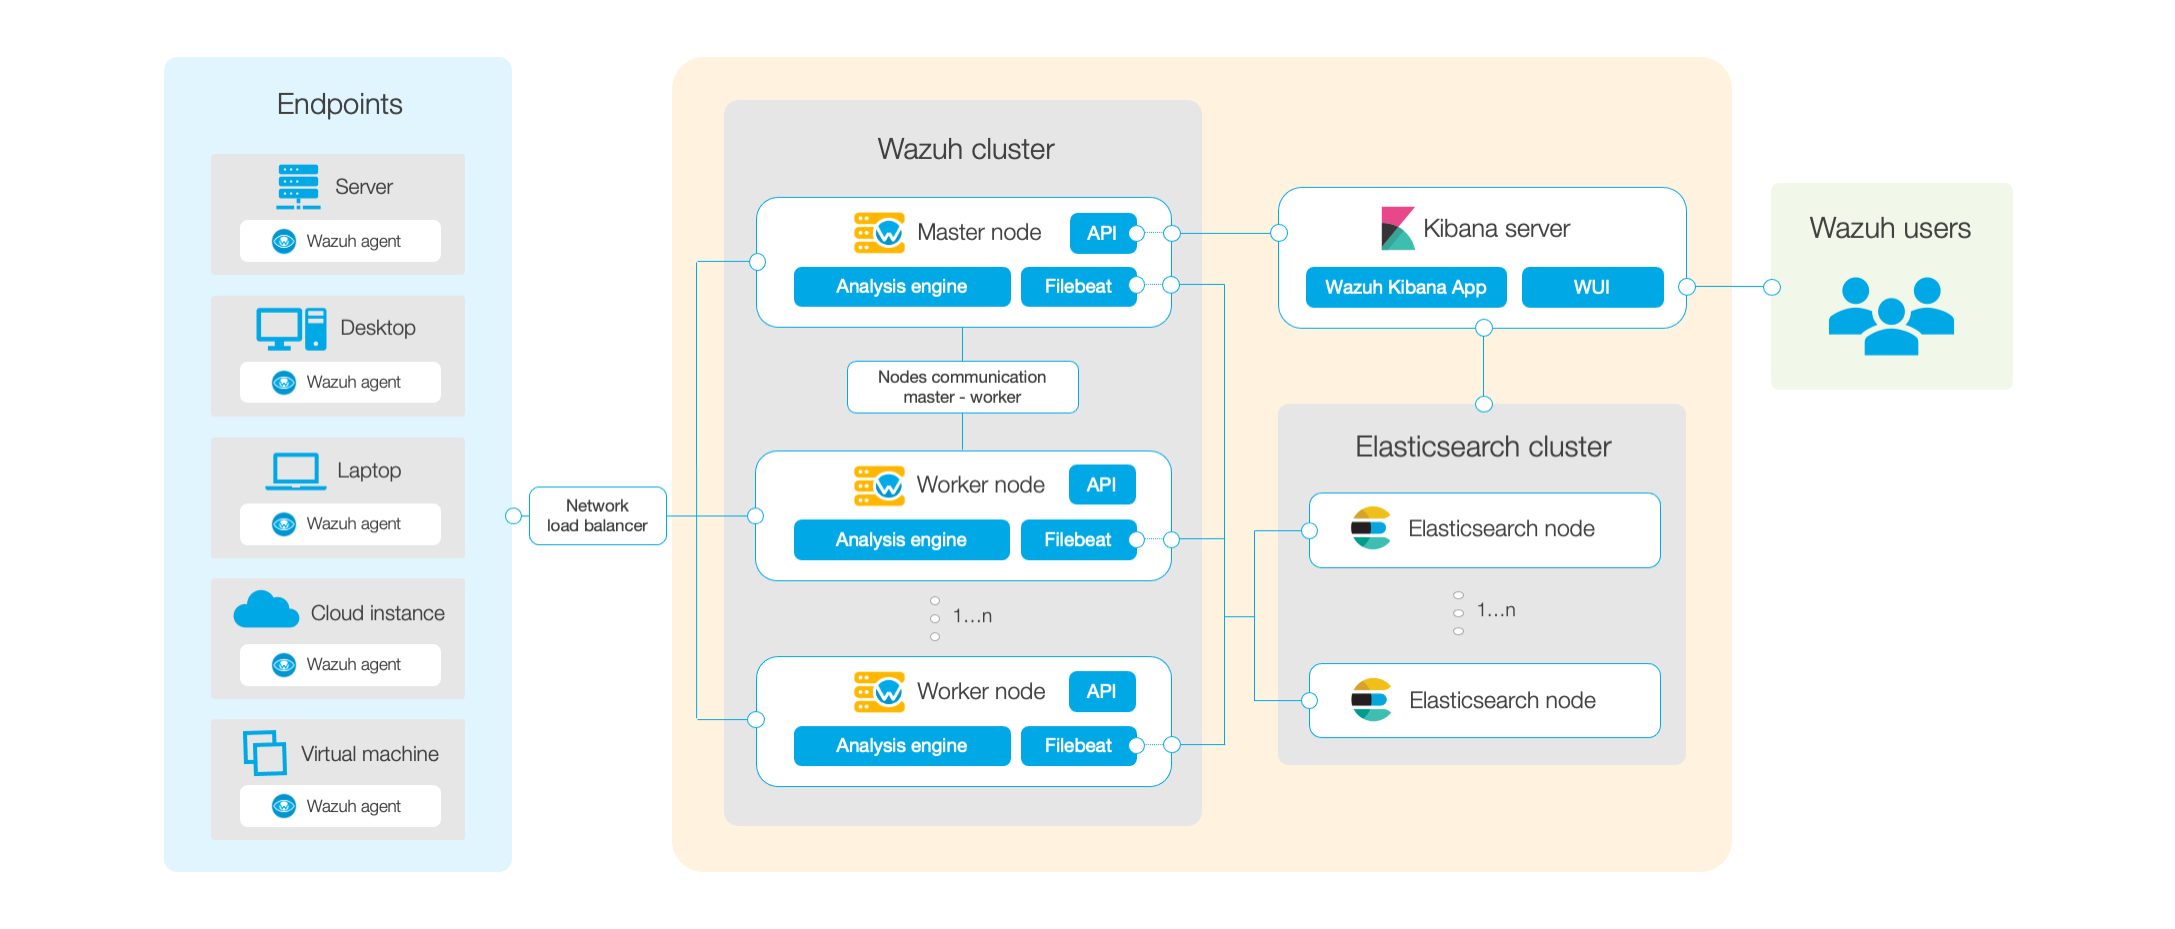
\includegraphics[width=\textwidth]{imagenes/wazuh_architecture.png}
  \caption{Esquema de la arquitectura de funcionamiento completo de Wazuh. Compuesta por uno o varios endpoints (que serán analizados por Wazuh), un cluster de gestores de Wazuh, un cluster de nodos de Elasticsearch y un servicio web Kibana con un plugin específico llamado `Wazuh Kibana App`. }
  \label{wazuh_architecture}
\end{figure}

Para entender mejor cómo funciona, debemos atender a su arquitectura (ver figura \ref{wazuh_architecture}). Wazuh tiene dos elementos esenciales: \textbf{un \textit{manager}, o gestor, y un agente}, que se comunican entre sí. 

El agente de Wazuh se instala en los \textbf{endpoints} o dispositivos informáticos a analizar y se encarga de \textbf{extraer información importante de esos sistemas}, esta extracción de información puede ser por muchas vías \textbf{dependiendo de cómo esté Wazuh configurado}. Por ejemplo, se puede extraer información del propio sistema operativo utilizando el módulo de \textbf{syscollector} o de eventos (borrado, modificación, creación) relacionados con ficheros importantes del sistema con el módulo de \textbf{syscheck o File Integrity Monitoring}, entre otros. Además, los agentes se pueden configurar para leer y redirigir los logs de aquellas aplicaciones que nos sean de interés al gestor, dónde se analizarán como corresponda.

\begin{figure}[!hbt]
  \centering
  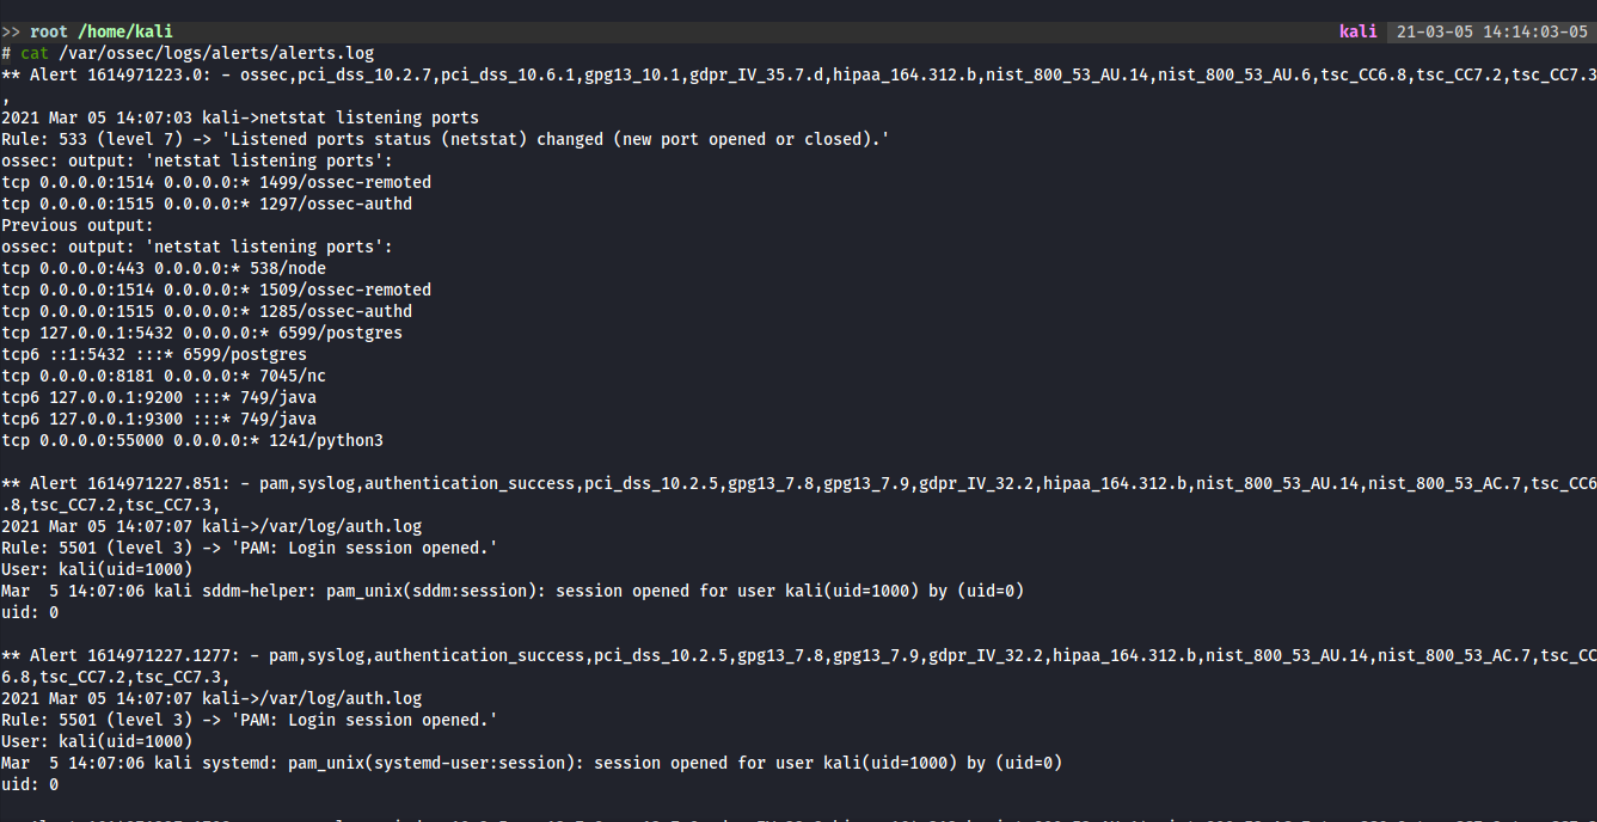
\includegraphics[width=\textwidth]{imagenes/alerts.png}
  \caption{Ejemplo de alertas en texto plano generadas por el gestor de Wazuh a partir de los eventos enviados por los agentes.}
  \label{wazuh_alerts}
\end{figure}


Por su parte, el \textit{Wazuh manager} recibe la información de los agentes. Parte de esta información es almacenada en bases de datos internas (información del OS, paquetes instalados, estados de los ficheros cuya integridad se está asegurando, etc...) y el resto es analizada (principalmente logs) y utilizada para generar \textbf{alertas de seguridad} (ver figura \ref{wazuh_alerts}). 

La información enviada por el agente se considera un \textbf{evento de seguridad} y es decodificada por el gestor para extraer los campos interesantes utilizando \textbf{decodificadores}. A continuación, la información extraída con dichos decodificadores pasa a través de unas \textbf{reglas} que determinan si se trata o no de un evento relevante, así como el tipo de evento, su grado de importancia, si está relacionado con alguna técnica de \gls{mitre}, etc. y ese evento pasa a ser una \textbf{alerta}, que se envía a la aplicación web por medio de Elasticsearch y a aquellos puntos para los que se haya configurado Wazuh (email, SMS, slack, telegram, etc...), esta funcionalidad de alertas con información relevante puede ser de mucho interés para los hackers éticos, como ya se ha explicado.

Es interesante comentar que Wazuh comenzó utilizando Elasticsearch con su versión original, llegando a dar soporte a sus funcionalidades de pago (xpack), pero que en el último año ha comenzado a dar soporte a otra alternativa opensource que ofrece las mismas funciones de forma libre y gratuita (Opendistro).

Con el reciente cambio de licencia en el proyecto de Elasticsearch (\cite{licensechange}), debido en parte a una disputa con Amazon, el entorno de Software que, como Wazuh, utilizan Elasticsearch, se encuentra en un momento inestable. Recientemente, Amazon ha hablado de una versión de Elasticsearch que continúe con la licencia opensource previa, llamada OpenSearch, y mantenida por la propia organización \cite{OpenSearch}. Para este trabajo, se ha mantenido la integración de Wazuh con la versión original de Elasticsearch pero \textbf{es muy probable que en un futuro cercano Wazuh se pueda integrar con otras alternativas}.

Estas reglas y decoders ya mencionados son parte del \textbf{ruleset} de Wazuh, y los usuarios pueden modificarlas o \textbf{crear la suyas propias} para extender la funcionalidad de Wazuh.

Una parte de este trabajo será analizar cómo recopilar datos de la auditoría de seguridad y enviarlos a Wazuh para que los analice como cualquier otro registro con información que llegue al gestor.

Entonces, utilizando la aplicación web de Kibana con \textbf{el plugin de Wazuh}, el usuario puede acceder a estos datos de alertas (así como a los datos disponibles en las bases de datos del gestor, a través de la API de Wazuh, por ejemplo para obtener información sobre los sistemas de los clientes), generar gráficos, tablas y reportes, hacer búsquedas según el valor de determinados parámetros, etc.

El objetivo último de poder generar y analizar información de las auditorías de seguridad con Wazuh sería \textbf{indexar esta información en Elasticsearch} de forma que pudiera ser fácilmente accesible, que se pudieran generar gráficos o reportes a partir de ella, etc.


\section{Definición de hacking ético}

De acuerdo con la guía de estudio del certificado de hacking ético (CEH) \cite{ceh}, un hacker ético (o penetration tester) es aquel que, con permiso explícito de una organización, utiliza sus habilidades como hacker para atacar los sistemas de la misma con el objetivo de descubrir vulnerabilidades. Un hacker ético no revela la información obtenida de dichos ataques a terceros y trabaja siempre con un contrato que garantice actuar dentro de los marcos legales.

Hoy día, también se denomina hacker éticos a aquellos que participan de los programas de \gls{bugb}, de los que ya se ha hablado anteriormente, y que comparen algunas metodologías y características con los tests de penetración de sistemas, pero en esencia son muy diferentes.

Para entender mejor qué es un hacker ético hay que compararlo con su opuesto: aquellos que aprovechan sus conocimientos sobre los sistemas informáticos para realizar actividades ilícitas sobre los sistemas de terceros, explotando sus vulnerabilidades con el objetivo de obtener algún beneficio. Estos individuos cometen delitos informáticos y van en contra de la ley. 

Dado que un hacker ético debe, por definición, actuar dentro del marco legal, es interesante que estudiemos los aspectos legales del hacking ético.

\section{Aspectos legales del hacking ético}

Es de vital importancia tener en cuenta la necesidad de un \textbf{permiso explícito} para realizar o no determinadas acciones en un sistema que no es nuestro.

Un hacker ético nunca debe hacer su trabajo sin permiso explícito de los responsable del sistema que va a probar y, aún teniendo permiso, debe limitar sus pruebas al ámbito que se establezca en el contrato de trabajo. Sobre esto hablaremos más adelante, cuando expliquemos las fases de las que consta un test de penetración de sistemas.

El porqué de estas medidas es que la ley ampara a cualquiera que sea dueño de un sistema informático y la intrusión en este sin permiso está penada en los principales gobiernos del mundo y, en concreto, en España (véase el Artículo 197 bis del Código Penal en España), dónde el acceso ilícito a un sistema de información sin permiso puede ser castigado con pena de presión de seis meses a dos años.

\begin{tcolorbox}[coltitle=blue!50!black,colframe=blue!25,title=Artículo 197 bis]
El que por cualquier medio o procedimiento, vulnerando las medidas de seguridad
establecidas para impedirlo, y sin estar debidamente autorizado, acceda o facilite a otro el
acceso al conjunto o una parte de un sistema de información o se mantenga en él en contra
de la voluntad de quien tenga el legítimo derecho a excluirlo, será castigado con pena de
prisión de seis meses a dos años.

\tcblower

Código Penal y legislación complementaria. Edición actualizada a \linebreak \textbf{17 de diciembre de 2020}
\end{tcolorbox}

\subsection{Convenios internacionales}

Dados que los crímenes relacionados con los sistemas de información pueden ser perpetrados desde cualquier lugar del mundo y, sin embargo, afectar a entidades de otras localizaciones, existen diversos \textbf{convenios internacionales} que indican a los países como proceder en situaciones de esta índole, que un hacker ético \textbf{debe tener en cuenta}, puesto que si se encuentra trabajando para una empresa extranjera podría verse afectado por las leyes de otros países además de las del suyo propio.

\subsubsection{Convenio 185 sobre la ciberdelincuencia}

En este convenio internacional se define el sistema informático como ` todo dispositivo aislado o conjunto de dispositivos interconectados o relacionados entre sí, cuya función, o la de alguno de sus elementos, sea el tratamiento automatizado de datos en ejecución de un programa.', es decir, desde un portátil personal hasta una \textit{smartTV} o un dispositivo \textit{IoT}. Esta definición se corresponde con la de \textbf{endpoint}, que ya hemos mencionado anteriormente y engloba al tipo de dispositivos que pueden ser protegidos por Wazuh.

Del mismo modo, se establecen los delitos contra la confidencialidad, integridad y disponibilidad de los datos y sistemas informáticos y se indica que \textbf{los países participantes deben adoptar las medidas legislativas necesarias para tipificar esos delitos}. Además, la segunda sección del Artículo 12  sobre la Responsabilidad de las personas jurídicas, indica que \textbf{se puede exigir responsabilidad a una persona jurídica cuando la ausencia de vigilancia o control haya propiciado un delito informático}. Todo esto está estrechamente relacionado con el uso de Wazuh en los sistemas que deben ser protegidos o, como se propone en el trabajo, como herramienta para monitorizar las acciones llevadas a cabo durante un test de penetración.

Y es que en cualquier momento un hacker ético puede verse envuelto en conflictos legales si ocurre algún problema durante una auditoría. Así pues, recalcamos la importancia de \textbf{registrar las acciones llevadas a cabo durante la auditoría} puesto que pueden servir como un complemento a la hora de demostrar qué cosas se han hecho o no durante la auditoría.

\begin{tcolorbox}[coltitle=blue!50!black,colframe=blue!25,title=Artículo 197 bis]
 Además de los casos previstos en el párrafo 1 del presente artículo, cada parte
adoptará las medidas necesarias para garantizar que pueda exigirse responsabilidad
a una persona jurídica cuando la ausencia de vigilancia o de control por parte de
cualquier persona física mencionada en el párrafo 1 haya permitido la comisión de un
delito...
\tcblower
Artículo 12 – Responsabilidad de las personas jurídicas del convenio 185 sobre la ciberdelincuencia \cite{t108}
\end{tcolorbox}


\subsection{Leyes y regulaciones a nivel Europeo}

Otro factor clave para entender la importancia de software como Wazuh y el papel que podría tener un especialista analizando el rendimiento de este en un entorno profesional son las regulaciones de seguridad que deben cumplir las empresas.

A nivel europeo existen varias regulaciones que \textbf{las empresas deben cumplir}. Entre ellas, destaca por ejemplo la regulación general de protección de datos (GDPR) que en España se aplica a través del reglamento general de protección de datos (RGPD) \cite{rgpd}, que regula toda la normativa relacionada con la recogida, tratamiento y almacenamiento de datos personales o sensibles como por ejemplo, la información sanitaria de un paciente en un hospital. 
Desde el punto de vista de un analista de ciberseguridad, lo más importante de esta ley son las implicaciones relacionadas con la protección de los datos almacenados. 

En España, basándose en la RGPD, existe la Ley Orgánica de Protección de Datos (LOPD) \cite{lopd}. Tanto la LOPD como la RGPD establecen como se deben tratar los datos personales en nuestros sistemas informáticos, sin embargo, existen unas medidas o normativas extra que las empresas con datos susceptibles de entrar en el marco de estas leyes deben cumplir según el ámbito en el que operen. Son las normativas como HIPAA, PCI DSS o SOC, en inglés comúnmente conocidas como `Compliances'.

Estas normativas se analizarán a continuación, así como sus implicaciones y su relación con software de seguridad como Wazuh.

\section{Normativas de ciberseguridad}

Además de las leyes que establecen los delitos informáticos, existen una serie de regulaciones o normativas propias de los distintos sectores financieros que las empresas que dispongan de determinado tipo de datos deben comprometerse a cumplir. Del inglés \Gls{compliance}, que podría traducirse como 'el cumplimiento' de las normativas o leyes referentes a la seguridad de los datos que una empresa pueda almacenar o gestionar. Cualquier compañía con acceso a datos sensibles de sus clientes está obligada a asegurar unos mínimos requisitos de seguridad en sus entornos y ser capaz de demostrar que los cumple \cite{phoenixnap}. 

Algunos ejemplos importantes de \textit{'compliances'} se enumeran a continuación.

\begin{description}
\item[HIPAA](Health Insurance Portability and Accountability Act) Se aplica a compañías del ámbito sanitario y regulariza cómo dichas compañías deben manejar y asegurar la seguridad de los datos médicos personales de sus pacientes. 

\item[PCI DSS] (Payment Card Industry Data Security Standard) Creado por algunas compañías de la industria de pago con tarjetas de crédito que quiso normalizar como se asegurar la integridad de la información financiera de sus clientes. Wazuh \cite{wazuh-pci} cuenta con herramientas para asegurar este \textit{compliance} asegurando (entre otros) la detección de \textit{rootkits}.

\item[SOC Reports] Se trata de unos reportes de control de sistemas y organizaciones verificable, llevado a cabo por una \acrfull{CPA} para asegurar el cumplimiento de las normativas de seguridad cuando la compañía maneja datos sensibles de sus clientes.

\end{description}

Una de las ventajas o funcionalidades que ofrece Wazuh a sus clientes es que dispone de las herramientas necesarias para asegurar el cumplimiento de estas normativas o estándares. En concreto, en su web\footnote{\url{https://documentation.wazuh.com/current/compliance.html}} se afirma que ofrece mecanismos para cumplir con las ya mencionadas \textbf{PCI DSS} y \textbf{GDPR}. Sin embargo, como se ha tratado de explicar varias veces en la introducción, Wazuh es una herramienta que debe ser configurada correctamente para poder abarcar todo su potencial. Es por ello que \textbf{no} bastaría con instalarla en un sistema para cumplir estas normativas y, \textbf{ante una auditoría gubernamental, una mala configuración podría suponer el incumplimiento de las normativas.}

Es por esto que debemos resaltar la importancia de analizar el rendimiento de Wazuh en cada entorno dónde se instala y valorar si realmente está cubriendo todas las amenazas que debe cubrir.

A continuación, se describen las principales fases de una auditoría de ciberseguridad y se ahonda en la importancia de los aspectos legales ya mencionados y en las posibilidades que ofrece incorporar Wazuh dentro del esquema de un test de penetración de sistemas.


\section{Fases de una auditoría de ciberseguridad}

Para poder llevar a cabo correctamente una auditoría de seguridad, primero necesitamos tener claros los pasos a seguir y para ello no hay mejor punto de partida que usar el estándar de \textbf{http://www.pentest-standard.org}. Distinguiremos 7 fases principales:
\begin{enumerate}
    \item Puesta a punto
    \item Recopilación de información
    \item Análisis de riesgos
    \item Análisis de vulnerabilidades
    \item Explotación de vulnerabilidades
    \item Post-explotación
    \item Elaboración de informe final
\end{enumerate}

A continuación se describen con mayor detalle cada una de las etapas.

\subsection{Puesta a punto (pre-engagement)}

La primera fase consiste en la puesta a punto del contrato con la empresa para definir el ámbito de la auditoría, responder a la preguntas siguientes, entre otras.

\begin{itemize}
    \item \textbf{¿Cuál es el objetivo de la auditoría?}
    \item \textbf{¿De cuánto tiempo se dispone?}
    \item \textbf{¿Qué se espera que probemos?} 
\end{itemize} 

Esto está estrechamente relacionado con los aspectos legales ya descritos: salirse del marco establecido podría incurrir en problemas legales y en consecuencias para el auditor. Es por ello que disponer de herramientas adecuadas para registrar sus acciones y \textbf{compartirlas en tiempo real con los clientes} puede suponer una enorme ventaja para los profesionales del sector.

\subsection{Recopilación de información}

La segunda fase es la recopilación de toda la información posible sobre los objetivos con el objetivo de descubrir los puntos de acceso al sistema: IPs de los distintos servidores, servicios utilizados por estos y abiertos a peticiones externas, websites, etc..., así como posible vulnerabilidades relacionadas con los usuarios del mismo (correos electrónicos que podrían ser hackeables, contraseñas inseguras o nombres de usuario que aparezcan en bases de datos de la deep web, etc...), esto también incluye vulnerabilidades físicas (localización de oficinas, servidores, etc... y la seguridad de las mismas, por ejemplo).

Dependiendo de lo que se establezca en el contrato la auditoría podrá abarcar la seguridad física de la empresa (acceso a oficinas y sus dispositivos, servidores, documentos físicos...) o limitarse al ámbito informático, en este caso, la recopilación de información incluye el mapeo de redes públicas (y privadas si se tiene acceso) y la enumeración de hosts, DNS, servicios, puertos, dominios, etc... usando herramientas como \textbf{nmap}, metasploit\cite{kennedy_2011}, wireshark, etc...

Respecto al uso de Wazuh como complemento durante esta fase es interesante mencionar, por ejemplo, que herramientas como \textbf{nmap} disponen de opciones para hacer sus análisis más `agresivos' o más discretos, con el fin de encontrar un balance entre la información obtenida y la exposición del propio análisis ante las herramientas de protección de los sistemas. Es por ello que a veces debemos realizar los análisis de puertos o enumeraciones de servicios de forma más lenta y prolongada en el espacio o utilizando mecanismos para enviar mensajes desde distintos orígenes \textbf{con el objetivo de que el análisis no sea descubierto}. Por tanto, tener un registro de los resultados obtenidos nos permite evitar realizar el mismo análisis varias veces, poder fácilmente compartirlo con compañeros de equipo o con los clientes (a la hora de enviar un reporte, por ejemplo) etc.. Si bien estas herramientas suelen disponer de opciones para exportar sus resultados en formatos almacenables y analizables por otros programas, disponer de un motor de indexación como Elasticsearch, con ayuda de Wazuh, puede ser muy útil en esta fase del test.

\subsection{Modelización de amenazas o análisis de riesgos}

A continuación y partiendo de la información recopilada en la fase anterior deberíamos diseñar un modelo de amenazas. ¿Qué creemos que es susceptible de ser atacado? ¿Por qué? Dependiendo de cómo sea la compañía que nos contrata y, poniéndonos en la piel de un posible atacante, debemos elegir cuales serían nuestros objetivos, si obtener información o datos personales de clientes o de los propios trabajadores de la empresa, robar algún tipo de información de la empresa, romper o inhabilitar algún servicio de la misma... Por poner un ejemplo: dentro de una empresa los objetivos de un atacante serían muy distintos si se trata de una clínica o de una tienda online. En el primer caso probablemente buscaríamos acceso a datos confidenciales de los clientes y en el segundo quizá buscáramos obtener beneficios de la tienda online o desarticularla temporalmente. En esta fase también es importante tratar de entender las posibles razones que existirían para cometer estos delitos. Tratar de buscar una justificación o una explicación para estas amenazas. ¿Podemos obtener algún beneficio de los datos robados? ¿Nos interesa que esta web deje de funcionar para que sus clientes se muevan a otra plataforma? Preguntas como esta son las que deben plantearse y responderse.

\subsection{Análisis de vulnerabilidades}

Esta es la fase en la que se buscan defectos y vulnerabilidades en los sistemas de la empresa. En el ámbito informático es dónde se analizan los servicios ofrecidos por los sistemas de la misma y se buscan vulnerabilidades en ellos. Para ello, principalmente se utilizan herramientas y bases de datos de vulnerabilidades. Por ejemplo, utilizando el framework de scripts de nmap, o mestasploit, utilizando herramientas para SQL injection automática (como JSQL), web fuzzers (\Gls{Fuzzing}) , etc...


\subsection{Explotación de vulnerabilidades}

Una vez encontradas y analizadas las principales vulnerabilidades de la organización, el siguiente paso sería tratar de explotar las mismas con el objetivo de encontrar un punto de acceso dentro del entorno de la organización o a algún elemento de la misma (bases de datos, directorios activos, etc...)

Esta fase es compleja y depende mucho del escenario. Un ejemplo de explotación de vulnerabilidades sería aprovechar falta de procesamiento de datos en una web para conseguir acceso a la base de datos por medio de SQL injection o aprovechar el uso de contraseñas débiles en correos electrónicos para acceder a información de la empresa por medio de fuerza bruta.

\subsection{Post-explotación}

Si se consigue acceso a una máquina o base de datos, en una fase posterior, analizaremos la importancia de este logro (que viene determinada por la cantidad y calidad de la información disponible en esta máquina, así como de su utilidad para comprometer el resto de redes privadas de la organización a las que tenga acceso). 

Aquí se incluyen labores de persistencia (asegurar la posibilidad de volver a acceder al sistema comprometido), penetración adicional o escalado de privilegios, entre otros. Hay que tener en cuenta que Wazuh es una herramienta que puede utilizarse para labores de {\it \gls{forensics}} y, desde el punto de vista de un atacante, es importante utilizar mecanismos de ocultación o {\it \gls{antiforensics}} para entorpecer las labores de herramientas como Wazuh. En este caso, querríamos registrar dichos intentos de ocultación con el módulo desarrollado, para relacionarlo con lo que es capaz de detectar Wazuh por sí mismo.

\subsection{Elaboración de informe}

Finalmente, se desarrolla un reporte o informe de la auditoría. Debe tener dos secciones bien diferenciadas: un informe para ejecutivos, orientado a directivos de la empresa posiblemente sin conocimientos técnicos, y otro informe técnico para el personal informático de la empresa.

Se debe incluir toda la información desarrollada en las fases anteriores así como un análisis y clasificación de las vulnerabilidades demostradas según su importancia y según \textbf{los activos que sean comprometidos por ellas}.

El reporte es uno de los puntos en los que puede ser clave contar con la información indexada por Wazuh, podríamos por ejemplo usarla para crear gráficos, históricos y tablas, para fácilmente encontrar o adjuntar el output de ciertos comandos ejecutados, entre otros.
